\documentclass[12pt, a4paper]{article}

\usepackage{times}
\usepackage{mathptmx}
\usepackage{amsmath}
\usepackage{graphicx}
\usepackage{setspace}
    \doublespacing
\usepackage{floatrow}
\usepackage{tikz}
    \usetikzlibrary{calc, shapes, backgrounds}
\usepackage{amssymb}
\usepackage[boxed, linesnumbered, lined]{algorithm2e}
\usepackage{pgfplots}
    \pgfplotsset{compat=1.12}

\begin{document}

    \title{\bf Introduction to $K$-Dimensional Tree}
    \author{
        {Pingchuan Ma\thanks{Student ID: 1511442}}\\
        College of Software, Nankai University\\
        {\tt pika7ma@gmail.com}
    }
    \date{}
    \maketitle

    \hrule

    \begin{abstract}
        \noindent
        {\sl This state-of-the-art report summarizes $k$-dimensional tree research and further applications within computer science.}\\
        {\bf Keywords:} Data Structure, $K$-dimensional Tree, Combinatorics
    \end{abstract}

    \hrule

    \section{Introduction}
        $K$-dimensional tree \cite{Bentley:1975:MBS:361002.361007} (or $k$-d tree, where $k$ is a random integer indicates the dimensionality of the search space) has been established as one of the major solutions to modelling multidimensional space. While $k$-d tree initially gained popularity as multidimensional data structure, it has emerged to play a role in other fields (e.g.\ particle simulation and clustering). $K$-d tree is also a special case of binary space partitioning tree.\\

    \section{The Method}
        Given a low dimensional continuous space, the basic idea of $k$-d trees is attempting to cut this space into halves and limiting the searching into one of the quadrants to reduce the computational complexity.

        To simplify the problem in order to provide insight into this artful but confusing data structure, the sample dimensionality has been set into 2D. Consider this training data set:
        \begin{equation*}\begin{split}
            \{&(1, 9), (2, 3), (4, 1), (3, 7), (5, 4),\\
              &(6, 8), (7, 2), (8, 8), (7, 9), (9, 6)\}
        \end{split}\end{equation*}

        Now the axes have two attributes. The algorithm works like that we pick an attribute and find the median, then we split the data set along that median. For example, in this case, the median happens to be 6 at the first time split, so we have the points in the upper line on the left side and the lower ones on the right. Similarly, we do the same things to the second attributes, then we work out a tree-like data structure. The pseudocode is followed:

        \begin{algorithm}[ht]
            \KwData{axis, median: integer}
            {\bf function} kdtree(pointSet, depth)\\
            \Begin{
                axis $\gets$ depth mod k\;
                median $\gets$ selected based on axis from pointSet\;
                newNode.location $\gets$ median\;
                newNode.left $\gets$ kdtree(points {\bf in} pointSet {\bf before} median, depth + 1)\;
                newNode.right $\gets$ kdtree(points {\bf in} pointSet {\bf after} median, depth + 1)\;
            }
        \end{algorithm}

        As a result, we are going to fracture the space into some little cubes and hypercubes. When it comes to inserting, every time we get a new data point, we can just walk down the tree until we end up in one of these hypercubes.

        \begin{figure}[ht]
            \begin{floatrow}[1]
                \ffigbox{\caption{Building a $k$-d tree from training data.}} {
                    \tikzset{
                        up/.style = {fill = orange!90!blue,
                            label = center:\textsf{\Large X}},
                        down/.style = {fill = blue!70!yellow, text = black,
                            label = center:\textsf{\Large Y}}
                    }
                    \begin{tikzpicture}[
                        scale = 0.8, transform shape, thick,
                        every node/.style = {draw, circle, minimum size = 10mm},
                        grow = down,  % alignment of characters
                        level 1/.style = {sibling distance=3cm},
                        level 2/.style = {sibling distance=6cm},
                        level 3/.style = {sibling distance=4cm},
                        level distance = 2cm
                    ]
                    \node[shape = rectangle, rounded corners, minimum width = 4cm] {The Training Data}
                    child{
                        node[up](Start){}
                        child{
                            node [down] (A) {}
                            child{
                                node [shape = rectangle, rounded corners, text width = 10mm] (B) {
                                    (2, 3) (4, 1)
                                }
                            }
                            child{
                                node [shape = rectangle, rounded corners, text width = 10mm] (C) {
                                    (1, 9)
                                    (3, 7)
                                    (5, 4)
                                }
                            }
                        }
                        child{
                            node [down] (D) {}
                            child {
                                node [shape = rectangle, rounded corners, text width = 10mm] (E) {
                                    (7, 2)
                                    (9, 6)
                                }
                            }
                            child {
                                node [shape = rectangle, rounded corners, text width = 10mm] (F) {
                                    (6, 8)
                                    (7, 9)
                                    (8, 8)
                                }
                            }
                        }
                    };

                    % Labels
                    \begin{scope}[nodes = {draw = none}]
                        \path (Start) -- (A) node [near start, left]  {$<6$};
                        \path (A)     -- (B) node [near start, left]  {$<4$};
                        \path (A)     -- (C) node [near start, right] {$\geq4$};
                        \path (Start) -- (D) node [near start, right] {$\geq6$};
                        \path (D)     -- (E) node [near start, left]  {$<8$};
                        \path (D)     -- (F) node [near start, right] {$\geq8$};
                    \end{scope}
                \end{tikzpicture}
            }
        \end{floatrow}
    \end{figure}

    Apparently, $k$-d tree is an approximate technique that you may make mistakes when implementing searching, but it allows you to quickly drill down to a bucket that has roughly correct position.

    \section{Applications}

    \subsection{Clustering}
        Since our tree-like data structure is modeled based on a multidimensional space, intuitively, its main function will be implemented on space working. Clustering is a well-known phenomenon in geometric data, and has application in machine learning. To simplify the problem, we define the distance function in standardized euclidean metric:

        \begin{equation*}\begin{split}
            d(p,q)=d(q,p)&=\sqrt{(q_{1}-p_{1})^2+(q_{2}-p_{2})^2+\cdots+(q_{n}-p_{n})^2}\\
            &=\sqrt{\sum_{i=1}^{n}{(q_{i}-p_{i})^2}}
        \end{split}\end{equation*}

        In a low dimensionality, the quickly drilling feature of $k$-d tree enables it as a speeding up of $k$-means clustering \cite{DBLP:conf/sdm/Hamerly10} (Lloyd's algorithm is more efficient for higher dimension).

        \begin{figure}[ht]
            \floatsetup{floatrowsep = qquad}
            \begin{floatrow}[2]
                \ffigbox[\FBwidth]{\caption{One case in clustering.}}{
                    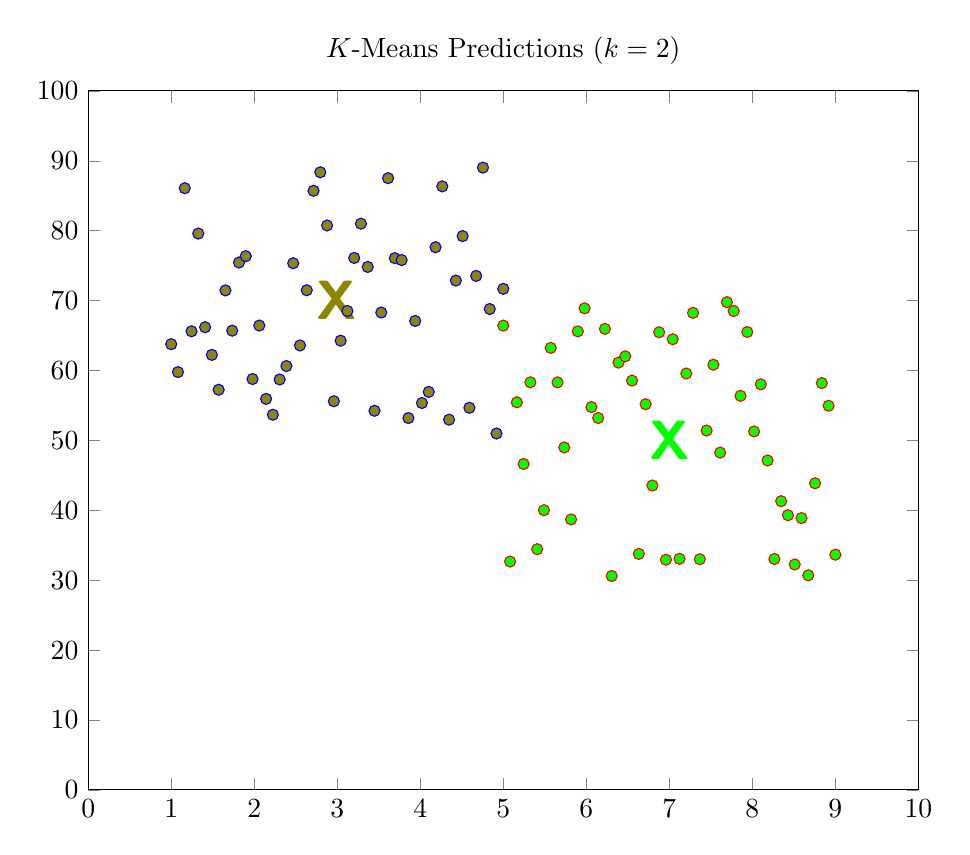
\begin{tikzpicture}
                        \begin{axis}[
                            width=\linewidth,
                            title={$K$-Means Predictions ($k=2$)},
                            xmin=0,xmax=10,ymin=0,ymax=100,
                            ]
                            \node[text=olive,font=\sffamily\bfseries,scale=2] at (3,70) {X};
                            \addplot+[y filter/.expression={y+50},only marks,mark=*, samples=50,mark
                            options={fill=olive},domain=1:5] {40*rnd};
                            \node[text=green,font=\sffamily\bfseries,scale=2] at (7,50){X};
                            \addplot+[y filter/.expression={y+30},only marks,mark=*,mark options={fill=green},samples=50,domain=5:9] {40*rnd};
                        \end{axis}
                    \end{tikzpicture}
                }
                \ffigbox[\FBwidth]{\caption{Another case in clustering.}}{
                    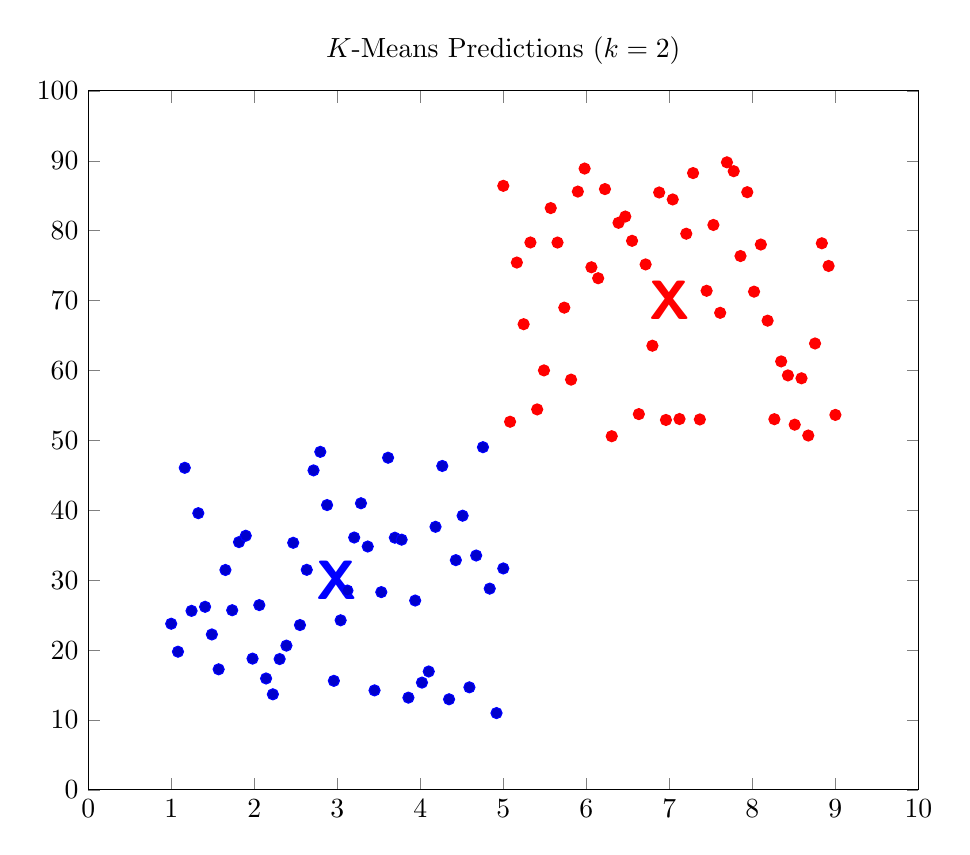
\begin{tikzpicture}
                        \begin{axis}[
                            width=\linewidth,
                            title={$K$-Means Predictions ($k=2$)},
                            xmin=0,xmax=10,ymin=0,ymax=100,
                            ]
                            \node[text=blue,font=\sffamily\bfseries,scale=2] at (3,30) {X};
                            \addplot + [y filter/.expression={y+10},only marks, mark=*,samples=50,domain=1:5] {40 * rnd};
                            \node[text=red,font=\sffamily\bfseries,scale=2] at (7,70){X};
                            \addplot+[y filter/.expression={y+50},only marks, mark=*,mark options={fill=red},samples=50,domain=5:9] {40*rnd};
                        \end{axis}
                    \end{tikzpicture}
                }
            \end{floatrow}
        \end{figure}

    \subsection{Particle Simulation}
        In computer graphics, we compute the movement of fluid particles with the help of multiple numerical methods which trying to solve the famous {\sl incompressible Navier-Stokes equation} \cite{bridson2015fluid}. It describes the motion of fluid substances as a result of forces.

        \begin{equation}
        \frac{\partial \overrightarrow v}{\partial t} + ({\overrightarrow v}\cdot{\overrightarrow \nabla}){\overrightarrow v} = \frac{-\overrightarrow \nabla p}{\rho_m} + \frac{\mu}{\rho_m}{ \nabla^2}{\overrightarrow v} + \frac{\overrightarrow f_{ext}}{\rho_m}
        \label{e1}
        \end{equation}
        \begin{equation}
        {\nabla v} = {0}
        \label{e0}
        \end{equation}

        Though it seems extremely complex at first glance, we have two intuitive approach to make it: Lagrangian and Eulerian viewpoint, which is particle-based and grid-based respectively.

        When it comes to the Lagrangian viewpoint, Smoothed Particle Hydrodynamics \cite{Muller:2003:PFS:846276.846298} (or SPH) has been considered as one of the major particle-based approach to simulate fluid. However, a space-fitting data structure is in need to search the neighbor particles in order to boost the kernel function used in SPH.

        Since then, plentiful applications of particle-based fluid simulation, such as Gasoline \cite{WADSLEY2004137}, have been done with the hierarchy data structure $k$-d tree in terms of the quickness of searching, deleting and inserting.

        \begin{figure}[ht]
            \centering
            \includegraphics[width=13cm]{sph.png}
            \caption{A sample SPH particle system.}
        \end{figure}

    \section{Connection to Combinatorics}

        After the brief introduction, we can find that $k$-d tree is an optimization of binary search tree and a special case of binary space partitioning tree. In terms of computer science, $k$-d tree has been built as a branch of the search tree structure which aims to reduce the complexity of searching, deleting, sorting and inserting. Similarly, when it comes to combinatorics, $k$-d tree is a part of graph theory which is one of the combinatorial concepts covered in our class. On one hand, $k$-d tree is an extended branch of tree in graph theory. On the other hand, the space partition is also a topic in combinatorics.

        Furthermore, in our continuous space in real world, it is pretty intuitive to deal with and judge the different part of space. However, to computer, which has no sight and is able to process discrete data merely, modeling the presentative but complicated problem into a batch of code or data somehow plays a vital role in computer science. From my point of view, combinatorics is a specific science that breaks up information into discrete state and designs algorithm to deal with them in a mathematical view. As a result, $k$-d tree can be abstracted as an imaginary hierarchy structure in abstract mathematics or even a clever pattern of designing discrete data.

    \section{Conclusion}

        This report concludes the background, basic principles, thinking patterns, implementations, applications and mathematical connections of $k$-d tree. Based on the coverage of combinatorial concepts during summer course and my independent reflection, this report can be qualified for a $k$-d tree primer and a learning stimulator for data structure and combinatorics. In the course of working out this report, I gained experience of manipulating the \LaTeX \ typesetting and programming language. Moreover, I gained an insight into combinatorics and data structure. Finally, I would like to extend my sincere gratitude to my combinatorics teacher during summer semester, Hua Wang, for his patient lectures and professional instruction.

    \bibliographystyle{acm}
    \bibliography{kdtree}

\end{document}
